\pagenumbering{arabic}
\setcounter{page}{1}
\fancyhead[l]{}
\nochapter{INTRODUCTION GENERALE}
\hspace{0.5cm}
\section*{Contexte et justifcation}
À l'ère du Big Data, l'analyse des masses de données constitue un enjeu majeur pour comprendre et optimiser les infrastructures numériques. Le Domain Name System (DNS), pierre angulaire d'Internet, représente un cas d'étude particulièrement pertinent dans ce contexte. Ce service fondamental, qui traduit les noms de domaine en adresses IP, est essentiel à la navigation fluide des utilisateurs sur Internet. Sans cette infrastructure, les utilisateurs seraient contraints de mémoriser des séries de chiffres complexes plutôt que des noms de domaine intuitifs, rendant l'accès aux ressources en ligne considérablement plus difficile.

\vspace{0.4cm}
L'infrastructure DNS mondiale traite quotidiennement des milliards de requêtes, générant un volume considérable de données exploitables. Les serveurs DNS publics de Google (8.8.8.8), largement utilisés à travers le monde, offrent un excellent terrain d'investigation pour analyser les performances d'un service critique. Malgré l'implémentation de techniques d'optimisation comme la mise en cache DNS, qui stocke temporairement les résultats des requêtes fréquentes, les performances des serveurs DNS continuent de montrer des variations significatives qui méritent une analyse approfondie, particulièrement dans un contexte où la dépendance aux services en ligne ne cesse de croître.


\vspace{0.4cm}
\section*{Problématique}
Dans un environnement où la rapidité et la fiabilité des infrastructures réseau sont essentielles, le serveur DNS public de Google (8.8.8.8) joue un rôle clé dans l’acheminement des requêtes internet. Cependant, des fluctuations de performance, notamment en termes de latence et de perte de paquets, peuvent affecter l’expérience utilisateur et la stabilité des connexions. Dès lors, quelles sont ces variations de performance et comment les expliquer ? Quels sont les facteurs influençant la stabilité du serveur et les périodes de dégradation des performances ?

\section*{Objectifs}
L'objectif principal de cette recherche est d'évaluer la performance du serveur DNS de Google, avec une attention particulière portée à la latence. De façon spécifique, nous visons à :
	\begin{itemize}
		\item Mesurer et analyser les fluctuations des temps de réponse du serveur DNS ;
		\item Évaluer les taux de perte de paquets et leur impact sur la connexion
		\item Evaluer la stabilité du routage des requêtes envoyées au serveur ;
		\item Analyser la stabilité et la variabilité des performances du serveur ;
		\item Identifier les périodes de latence élevée et leurs causes potentielles. ;
	\end{itemize}
	
\section*{Méthodologie et outils}
Notre démarche analytique s'articule autour d'une étude exploratoire initiale, utilisant des techniques de statistique descriptive pour caractériser les distributions des temps de réponse et autres métriques pertinentes. Nous approfondirons ensuite notre analyse en exploitant des outils adaptés au traitement de grands volumes de données comme PySpark, permettant une exploration plus fine des tendances et anomalies présentes dans notre jeu de données.

\vspace{0.4cm}
\section*{Plan du travail}
La première partie de cette étude concerne la présentation des données et l’analyse exploratoire. Dans cette section, nous allons décrire les données utilisées pour ces analyses et nous ferons  une breve analyses exploratoire. La deuxième partie de l'étude concerne une analyse approfondie de la base avec PySpark. Elle inclut  des statistiques descriptives, une analyse des variations du Time To Live (TTL) des requêtes DNS et la détection de tendances et d'anomalies, en utilisant des outils analytiques avancés pour obtenir des insights approfondis. La troisième partie est réservée à l’interprétation et à la discussion des résultats obtenus. Enfin, la dernière partie concerne la conclusion. 
%________________________________________________
\newpage
\chaptitle
\fancyhead[l]{}
\vspace{0.2cm}\ochapter{PRESENTATION DES DONNEES ET ANALYSES EXPLORATOIRES}\vspace{-0.7cm}


\section{Présentation des données}

\subsection{Source et nature des données}

Les données utilisées dans cette étude proviennent d'une commande \texttt{ping} exécutée pour mesurer la latence d'accès au serveur DNS public de Google (\texttt{8.8.8.8}). À chaque exécution de la commande, des paquets ICMP (Internet Control Message Protocol) sont envoyés à l'adresse cible à un intervalle d'une seconde. Chaque ligne de réponse représente l'état de la requête envoyée et contient des informations sur la latence ainsi que d'autres paramètres relatifs à la requête.

\subsubsection{Informations clés des données}

Chaque ligne contient plusieurs paramètres essentiels, qui fournissent des informations sur l'état de la requête ICMP envoyée ainsi que la latence observée. Les lignes peuvent être classées en plusieurs catégories selon l'état de la requête :

\begin{itemize}
	\item \textbf{Requête aboutie} : Représentée par une ligne contenant le temps de réponse en millisecondes (latence), comme par exemple \texttt{time=XXX ms}.
	\item \textbf{Requête non aboutie} : Certaines requêtes échouent, et la ligne contient un message indiquant l'échec de l'envoi, comme par exemple \texttt{ping: sendto: No route to host}.
	\item \textbf{Requête aboutie sans retour} : Dans certains cas, une requête peut atteindre la destination sans retour de données, résultant en un message de \texttt{Request timeout for icmp\_seq=XXX}, signifiant que la requête a été envoyée mais aucune réponse n'a été reçue dans le délai imparti.
\end{itemize}

\subsubsection{Structure d'une requête reussie (réponse)}

Une ligne représentant une requête réussie contient plusieurs informations structurées, qui permettent de mesurer et d'analyser la latence ainsi que d'autres caractéristiques du réseau. La structure d'une ligne typique de réponse réussie est la suivante :

\begin{itemize}
	\setstretch{1.3}
	\item \textbf{Taille du paquet reçu} : \texttt{64 bytes from 8.8.8.8} (indique que le paquet contient \textbf{64 octets} et provient de l'adresse IP cible).
	\item \textbf{Numéro de séquence ICMP} : \texttt{icmp\_seq=XX} (\textbf{XX} représente un identifiant unique incrémenté à chaque envoi).
	\item \textbf{TTL (Time-To-Live)} : \texttt{ttl=105} (indique le nombre maximal de sauts restants avant que le paquet soit rejeté).
	\item \textbf{Temps de réponse (latence)} : \texttt{time=XXX ms} (le temps \textbf{aller-retour} entre l'ordinateur source et l'adresse cible, exprimé en millisecondes).
\end{itemize}

Ces quatre éléments permettent de définir et d'analyser les caractéristiques d'une requête réussie, comme le temps que le paquet met à voyager entre l'ordinateur source et le serveur cible, ainsi que la fiabilité du réseau (indiquée par le TTL).

La date et l'heure de départ de la commande \texttt{ping} sont enregistrées dans la première ligne de la capture. Dans ce cas précis, la commande a été exécutée le :

\begin{itemize}
	\setstretch{1}
	\item \textbf{Date et heure de départ} : Vendredi 31 janvier à 09:23:12.
	\item \textbf{Adresse cible} : 8.8.8.8 (serveur DNS public de Google).
	\item \textbf{Intervalle de collecte} : Chaque seconde entre chaque requête envoyée.
\end{itemize}

\section{Analyses exploratoires}
Dans le cadre de l’analyse de la latence du serveur DNS public de Google (IP 8.8.8.8), un total de 80 222 requêtes ping ont été émises afin d’évaluer la stabilité et la performance de la connexion. Une brève exploration  a permis d’analyser le nombre de requêtes reçues avec succès, les erreurs rencontrées et les variations des TTL observées.

Sur les 80 222 tentatives, 76 529 requêtes ont bien été envoyées, tandis que 3 693 n’ont pas pu être émises, affichant une erreur "No Route to Host" ce qui signifie une absence de route valide vers la destination. Parmi les requêtes envoyées, 65 722 ont été traitées avec succès et ont reçu une réponse du serveur. En revanche, 10 807 requêtes ont atteint Google sans recevoir de réponse, générant une erreur "Request Time Out".

%_________________________________________________________________________________________
\newpage
\chaptitle
\fancyhead[l]{}
\vspace{-0.5cm}\ochapter{ANALYSES DE LA PERFORMANCE DU RESEAU AVEC PYSPARK}\vspace{0.4cm}
\hspace{0.5cm}

L’analyse de la performance réseau repose sur l’examen de plusieurs indicateurs clés permettant d’évaluer la stabilité et l’efficacité des connexions. Dans ce chapitre, nous exploitons PySpark pour traiter et analyser dix indicateurs de performance, offrant ainsi une vision détaillée des variations et des tendances observées.
\section{Indicateurs de tendance centrale }
L'analyse du temps moyen et de la médiane nous offre une vue d'ensemble sur la distribution des latences.
\begin{table}[H]	
	\captionsetup{justification=raggedright, singlelinecheck=false}
	\centering
	\caption{Mesures de tendance centrale}\vspace{-0.2cm}
	\setstretch{0.65}\fontsize{10}{20}\selectfont
	\begin{tabular}{||>{\raggedleft\arraybackslash}m{4cm}||c||}
		\hline
		\rowcolor{cyan}\textbf{Mesure} & \textbf{Valeur} \\
		\hline
		Médiane & 133.824 ms \\
		\hline
		Temps moyen & 634.931 ms \\
		\hline
	\end{tabular}
	\subcaption*{Source : Données collectées}
\end{table}
 Le temps moyen de 634.931 ms dépasse largement la médiane de 133.82 ms, ce qui indique une distribution asymétrique avec une queue droite étendue. Cela suggère la présence de latences extrêmes, c'est-à-dire des délais de réponse particulièrement longs, qui ont un impact significatif sur la moyenne. En revanche, la médiane, étant moins sensible aux valeurs aberrantes, fournit une meilleure indication de la latence centrale typique, représentant de manière plus fiable l'expérience de la majorité des requêtes.

\section{Indicateurs de  dispersion }
\begin{table}[H]	
	\captionsetup{justification=raggedright, singlelinecheck=false}
	\centering
	\caption{Mesures de dispersion}\vspace{-0.2cm}
	\setstretch{0.65}\fontsize{10}{20}\selectfont
	\begin{tabular}{||>{\raggedleft\arraybackslash}m{4cm}||c||}
		\hline
		\rowcolor{cyan}\textbf{Mesure} & \textbf{Valeur} \\
		\hline
		Premier quartile & 131.07 ms \\
		\hline
		Troisième quartile & 140.17875 ms \\
		\hline
		Temps maximal & 927,118.712 ms \\
		\hline
		Temps minimal & 35.597 ms \\
		\hline
		Ecart Type & 15,968.798 ms\\
		\hline
		\hline
	\end{tabular}
	\subcaption*{Source : Données collectées}
\end{table}
Le tableau présente des statistiques descriptives des temps de latence des requêtes ping vers le serveur DNS public de Google. On note :

\begin{itemize}
	\item Le premier quartile (131,07 ms) montre que 25 \% des requêtes sont rapides, sans congestion notable.
	\item La médiane (133,824 ms) indique une latence stable pour la moitié des requêtes.
	\item Le troisième quartile (140,17875 ms) suggère que certaines requêtes rencontrent des chemins plus lents ou des congestions.
\end{itemize}

Le temps minimal (35,6 ms) reflète une faible congestion, tandis que le temps maximal (927 118,712 ms) signale des paquets fortement retardés ou bloqués par des congestions sévères. L'écart type de 15 968,798 ms révèle une grande variabilité, indiquant des latences globalement rapides, mais avec des exceptions notables dues à des congestions temporaires ou des réacheminements.









\section{ Fréquences d'apparition des ttl}
\vspace{-0.5cm}
\begin{table}[H]	
	\captionsetup{justification=raggedright, singlelinecheck=false}
	\centering
	\caption{Nombre d'occurrences pour chaque TTL}\vspace{-0.2cm}
	\setstretch{0.65}\fontsize{10}{20}\selectfont
	\begin{tabular}{||>{\raggedleft\arraybackslash}m{3cm}||c||}
		\hline
		\rowcolor{cyan}\textbf{TTL} & \textbf{Nombre d'occurrences} \\
		\hline
		105 & 7 810 \\
		\hline
		100 & 61 \\
		\hline
		103 & 190 \\
		\hline
		114 & 52 883 \\
		\hline
		110 & 730 \\
		\hline
		109 & 4 048 \\
		\hline
	\end{tabular}
	\subcaption*{Source : Données collectées}
\end{table}
\vspace{-0.5cm}
Le tableau ci-dessus montre que dans la majeure partie des cas il y a environ 14 routeurs entre le serveur DNS de Google et l’émetteur des requetes. En effet, cette fréquence élevée du nombre d’occurrence du ‘TTL=114’ peut signifier qu’elle représente une route principale emprunter par les requêtes ou alors que la connexion utilise par l’émetteur est optimisée. 
\begin{figure}[H]	
	\centering 
	\caption{ Repartition du nombre d'occurence par TTL}
	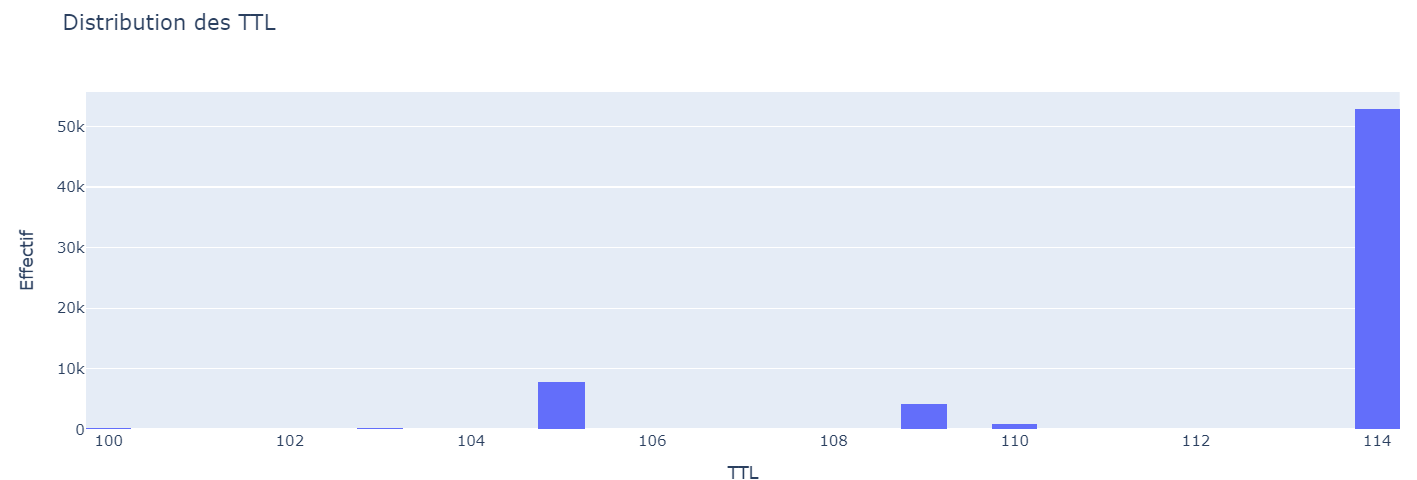
\includegraphics[width=0.75\textwidth, keepaspectratio]{Images/bar.png}
	\subcaption*{Source : \emph{Auteur a partir de python }}
\end{figure}
\vspace{-0.5cm}

\section{Taux de perte de paquets}
Le taux de perte de paquets est un indicateur essentiel pour évaluer la qualité d’une connexion réseau. Il représente le pourcentage de paquets envoyés qui ne parviennent pas à destination.
\vspace{-0.5cm}
\begin{figure}[H]	
	\centering 
	\caption{ Repartition des requêtes envoyées}
	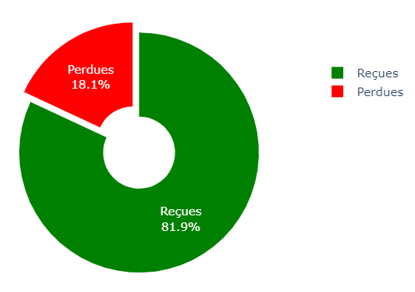
\includegraphics[width=0.45\textwidth, keepaspectratio]{Images/newplot.png}
	\subcaption*{Source : \emph{Auteur a partir de python }}
\end{figure}
\vspace{-0.5cm}
 Un taux de perte de 18.1 \% sur les requêtes envoyées est préoccupant et suggère l’existence de problèmes notables, potentiellement liés à la congestion du réseau, à des erreurs de configuration ou à des défaillances matérielles. Une investigation approfondie est nécessaire pour identifier précisément l'origine de ces pertes et mettre en place des mesures correctives adaptées.
\section{Moyenne par groupe de secondes}
\subsection{Par groupe de 10 secondes}
\vspace{-0.5cm}
\begin{figure}[H]	
	\centering 
	\caption{ Temps moyen par groupe de 10 secondes}
	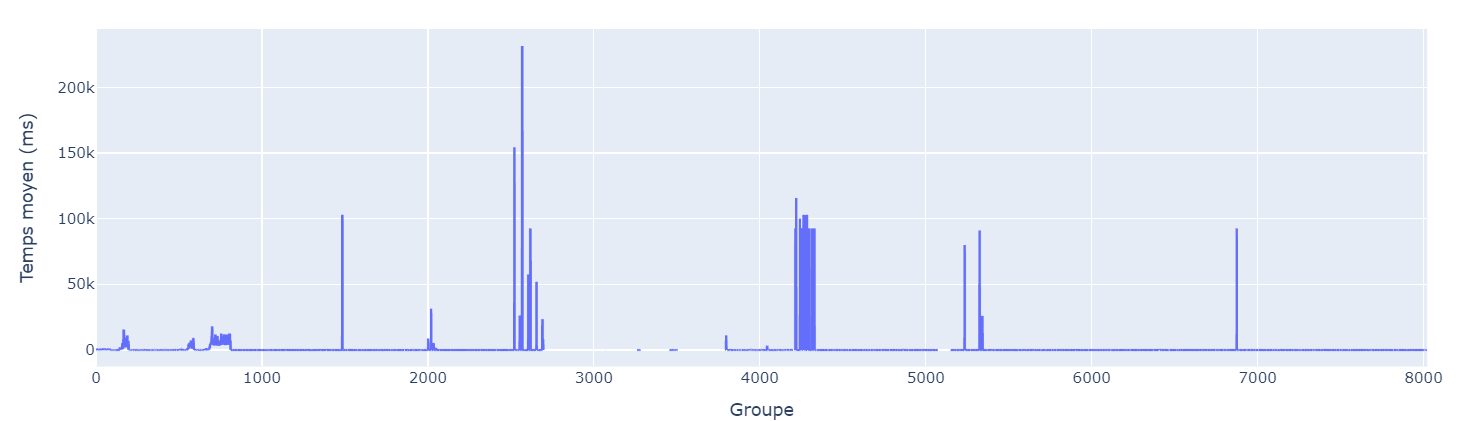
\includegraphics[width=1.05\textwidth, keepaspectratio]{Images/moy10.png}
	\subcaption*{Source : \emph{Auteur a partir de python }}
\end{figure}
\vspace{-0.5cm}

\subsection{Par groupe de 100 secondes}
\vspace{-0.5cm}
\begin{figure}[H]	
	\centering 
	\caption{ Temps moyen par groupe de 100 secondes}
	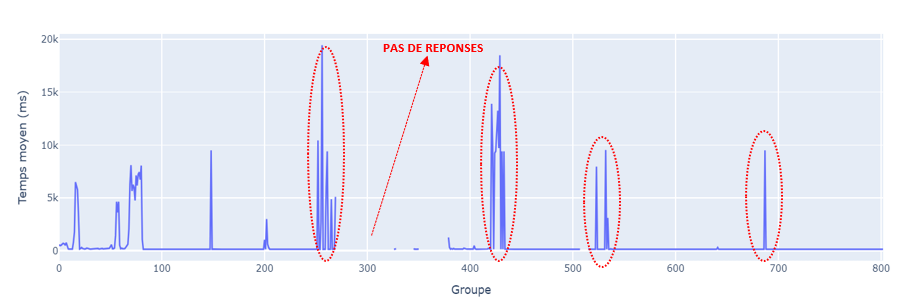
\includegraphics[width=1.05\textwidth, keepaspectratio]{Images/moy.png}
	\subcaption*{Source : \emph{Auteur a partir de python }}
\end{figure}
\vspace{-0.5cm}
Les graphiques ci-dessus fait état des niveaux moyens des temps de latence des requêtes par intervalle de 10 et 1000 secondes. On peut remarquer que une grande partie  du temps, la connexion semble avoir un comportement plus ou moins stable. Cependant, on observe plusieurs zones globalement repartie sur la période d’étude durant lesquelles les temps moyens des trajets des requêtes sont extrêmement au-dessus de la normale. Ces anomalies pourraient s'expliquer par une congestion temporaire du réseau, des politiques de filtrage ICMP appliquées par Google.

L'abscense de temps de latences sur le graphique correspond aux periodes pour lesquelles aucune réponse n'a été reçue. Cela signifie qu'aucune latence n'a pu être observée, ce qui peut être dû à plusieurs facteurs :

\begin{itemize}
	\item \textbf{Perte de paquets} : Les requêtes envoyées n'ont pas abouti à une réponse en raison de pertes dans le réseau, causées par une congestion, des erreurs de transmission ou des problèmes de routage.
	\item \textbf{Timeouts} : Les délais de réponse peuvent avoir dépassé un seuil défini, entraînant une absence d'enregistrement des latences.
	\item \textbf{Blocage ou filtrage des requêtes} : Certains pare-feu ou politiques réseau peuvent empêcher les réponses d'être envoyées, créant ainsi des périodes sans données.
	\item \textbf{Défaillance du serveur cible} : Si le serveur destinataire est temporairement indisponible ou en surcharge, il peut ne pas répondre aux requêtes.
\end{itemize}

\section{ le nombre de requetes où la latence est anormalement élevée}
L'analyse des latences montre que 9 685 requetes  présentent des valeurs anormalement élevées, identifiées comme valeurs aberrantes selon la règle de l'intervalle interquartile (IQR).Le temps de latence correspondant est supérieur 153.84 secondes

\section{ le nombre de requetes où la latence est anormalement faible, relativement à l'ensemble}
L'analyse des latences montre que 9 685 occurrences présentent des valeurs anormalement élevées, identifiées comme valeurs aberrantes selon la règle de l'intervalle interquartile (IQR).Le temps de latence correspondant est inférieur à 117.4 secondes
L'observation de \textbf{71 occurrences} avec une latence anormalement basse, identifiées comme \textbf{valeurs aberrantes inférieures}, suggère plusieurs scénarios possibles :

\begin{itemize}
	\item \textbf{Optimisation ponctuelle du réseau} : Certaines requêtes ont pu bénéficier d'une transmission ultra-rapide en raison d'un faible trafic ou d'une proximité avec le serveur.
	\item \textbf{Mécanismes de mise en cache} : Si certaines requêtes sont servies via un cache, elles peuvent afficher des temps de réponse bien inférieurs à la normale.
\end{itemize}

\section{Anomalies où le temps de latence dépasse un certain seuil}
\noindent Ces données révèlent une forte variabilité des temps de réponse du réseau, avec un nombre significatif de requêtes présentant des latences élevées :

\begin{itemize}
	\item \textbf{3 257 requêtes} ont dépassé \textbf{500 ms}, signalant déjà une dégradation notable des performances.
	\item \textbf{1 144 requêtes} ont dépassé \textbf{5 000 ms}, indiquant des délais critiques affectant gravement l'expérience utilisateur.
	\item \textbf{57 requêtes} ont excédé \textbf{15 000 ms}, traduisant des temps d'attente extrêmement longs.
	\item \textbf{30 requêtes} ont franchi \textbf{20 000 ms}, ce qui suggère des quasi-échecs de transmission ou des congestions réseau sévères.
\end{itemize}

\section{Repartition des TTL en fonction des seuil de latence anormales}
\begin{figure}[H]	
	\centering 
	\caption{Repation des TTL en fonction du temps de latence}
	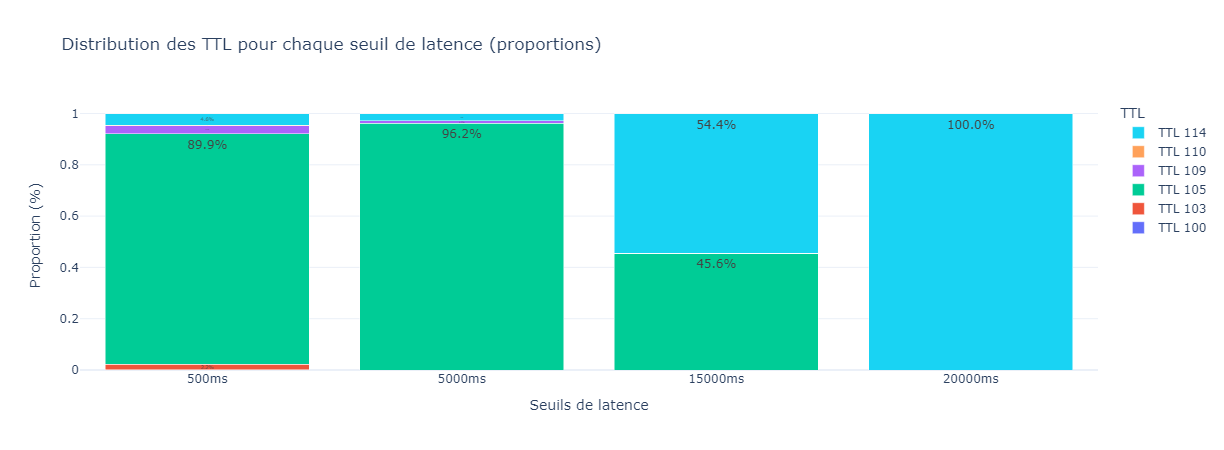
\includegraphics[width=1.05\textwidth, keepaspectratio]{Images/ttl.png}
	\subcaption*{Source : \emph{Auteur a partir de python }}
\end{figure}
Le diagramme présente la répartition des occurrences de TTL en fonction de niveaux de 
latence précis. Il apparaît clairement qu’à mesure que le temps de latence augmente, la 
proportion de requêtes avec un TTL de 114 devient de plus en plus prépondérante. Cette 
tendance, d’une part, confirme que le TTL 114 est l’occurrence la plus fréquente parmi 
l’ensemble des requêtes, et d’autre part, qu’il est fortement associé à des latences élevées.

Cette prépondérance suggère que la voie empruntée par les requêtes affichant un TTL de 114 
est probablement saturée. En effet, la concentration de requêtes à haute latence sur ce TTL 
laisse penser que le réseau rencontre une congestion sur cette route, ce qui ralentit le 
traitement des requêtes et accroît leur temps de latence.



\section{Variation moyenne  du délai de transmission des paquets ou gigue}
La gigue, ou \textit{jitter}, mesure la variation du délai de transmission des paquets dans un réseau. Elle est particulièrement importante pour les applications en temps réel, telles que le streaming vidéo, où une forte variabilité des délais peut entraîner une dégradation de la qualité de service.
La variation moyenne entre les valeurs de RTT successives est donnée par :
\begin{equation}
	Jitter = \frac{\sum |RTT_i - RTT_{i-1}|}{N-1}
\end{equation}
où \( RTT_i \) (Round-Trip Time) est le temps qu'un paquet met pour aller d'un émetteur à un récepteur et revenir lors de la \( i \)-ème requête envoyée, et \( N \) est le nombre total de requêtes.

D'après https://www.iptis.fr/blog/comprendre-la-qualite-de-sa-connexion-internet, une gigue inférieure à 20 ms est considérée comme optimale pour garantir une connexion stable et fluide. Or, dans notre cas, elle atteint 500.122 ms, une valeur extrêmement élevée qui indique une forte variabilité des délais entre les paquets de données. Une telle gigue peut entraîner des temps de réponse imprévisibles et dégrader significativement l'expérience utilisateur, rendant la navigation sur Internet lente et irrégulière. Cette instabilité résulte d’une fluctuation importante du temps que met chaque paquet pour traverser le réseau, avec des écarts pouvant aller de 0 à 500 ms, compromettant ainsi la qualité des services nécessitant un délai minimal, comme  le streaming en temps réel.



%_________________________________________________________________________________________
\newpage
\chaptitle
\fancyhead[l]{}
\vspace{0.2cm}\ochapter{INTERPRETATION ET DISCUSSION DES RESULTATS}\vspace{0.4cm}

Dans le cadre de l'évaluation de la latence du serveur DNS public de Google (IP 8.8.8.8), 80 222 requêtes ping ont été émises afin d'analyser la stabilité et la performance de la connexion. L'étude a permis d'examiner les requêtes réussies, les erreurs rencontrées et les variations des TTL observées.

\section{Statistiques générales sur l'émission et la réception des requêtes}
Sur les 80 222 requêtes envoyées, 76 529 ont été transmises avec succès, tandis que 3 693 ont échoué en raison de l'erreur \textit{"No Route to Host"}, indiquant une absence de route valide vers la destination. Parmi celles qui ont été envoyées, 65 722 ont reçu une réponse du serveur, tandis que 10 807 ont atteint le serveur sans réponse, générant l'erreur \textit{"Request Time Out"}.
Les erreurs \textit{"Request Time Out"} peuvent s’expliquer par plusieurs facteurs :
\begin{itemize}
	\item Filtrage ICMP appliqué par Google, qui pourrait ignorer certaines requêtes.
	\item Congestion réseau, entraînant une perte de paquets.
	\item Mécanismes de limitation du trafic ICMP mis en place par Google pour éviter les abus.
\end{itemize}

Les erreurs \textit{"No Route to Host"} sont plus probablement liées à des interruptions réseau côté client, une perte de connectivité temporaire ou un problème de routage externe.

\section{Analyse des TTL et de la stabilité du routage}
L’étude des TTL montre que 80\% des requêtes ont un même TTL, ce qui indique une route réseau stable et prédominante pour la majorité du trafic. Les 20\% restants affichent des TTL différents, suggérant :
\begin{itemize}
	\item L’existence de routes alternatives occasionnelles utilisées en cas de congestion.
	\item Des ajustements dynamiques du routage pouvant impacter certaines requêtes.
	\item Une instabilité intermittente sur certains segments du réseau.
\end{itemize}

Toutefois, la grande majorité des requêtes suivant une route fixe suggère que le routage dynamique n’est pas un facteur clé dans les variations de latence. Les fluctuations observées sont donc plus probablement liées à des problèmes de congestion réseau, de gestion des priorités ICMP ou de filtrage par Google.

\section{Analyse des temps de latence}
Les statistiques descriptives des latences révèlent une grande variabilité des temps de réponse. Bien que le temps médian soit de 133.8 ms, la moyenne est nettement plus élevée (634.9 ms) en raison de valeurs extrêmes pouvant atteindre 927 118 ms. Cette dispersion des latences peut être expliquée par :
\begin{itemize}
	\item Des pics de congestion réseau à certaines périodes, augmentant le délai de transmission.
	\item Des routes alternatives plus longues, utilisées temporairement pour certaines requêtes.
	\item Un traitement différentiel des paquets ICMP par Google, pouvant pénaliser certaines requêtes.
\end{itemize}

En observant l’évolution des latences par intervalle de temps, plus de 75\% des requêtes présentent une stabilité relative, mais certaines périodes montrent des augmentations brutales des délais, probablement dues à des interférences ou une congestion temporaire du réseau.



%_________________________________________________________________________________________

\newpage 
\fancyhead[l]{}
\pagenumbering{roman}
\renewcommand{\thepage}{\MakeUppercase{\roman{page}}}
\setcounter{page}{5}
\newpage 
\vspace{0.2cm}\nochapter{CONCLUSION }\vspace{0.4cm}

En conclusion, cette étude montre que la connexion au serveur DNS public de Google est généralement stable, comme le témoigne la constance du TTL pour près de 80 \% des requêtes. Cette stabilité suggère l’utilisation prépondérante d’une route principale, garantissant une connectivité fiable. Toutefois, les anomalies détectées — illustrées par des erreurs "Request Time Out" et "No Route to Host", ainsi que des pics de latence notables — indiquent que des fluctuations temporaires se produisent. Ces dernières sont probablement dues à des congestions réseau, à des mécanismes de filtrage ICMP ou à des réacheminements dynamiques. Bien que la majorité des requêtes aient donné de bons résultats, ces observations soulignent la nécessité d’une surveillance continue et d’analyses approfondies pour identifier et résoudre les défaillances potentielles du réseau. En définitive, cette investigation constitue une base solide pour comprendre les facteurs influençant la latence et offre des pistes concrètes pour optimiser la qualité du service DNS, notamment en traitant les interruptions intermittentes et en assurant l’efficacité du réseau.

%_________________________________________________________________________________________
\newpage
%\nocite{*}
%\vspace{0.2cm}\nochapter{BIBLIOGRAPHIE  ET WEBOGRAPHIE}\vspace{0.4cm}
%\renewcommand{\bibname}{klnoza} 
%\renewcommand{\refname}{}
%\printbibliography[heading=none]% none fait en sorte que cela ne cre pas ue nouvelle page

%________________________________________________________________________

